%!TEX root = ../main.tex

\section{Conditional Diversification Benefit} % (fold)
\label{sec:conditional_diversification_benefit}

This section studies a new measure of diversification in a portfolio called \emph{conditional diversification benefit} (CDB), which is developed by \textcite{ChristoffersenErrunzaJacobLanglois2012}. CDB is based on the portfolio expected shortfall (ES), i.e. the expected loss in case the return realizes below its Value-at-Risk (VaR), and therefore concerns the properties of the lower tail of the portfolio distribution.

If factors are not multivariate normal, the covariance matrix used in mean-variance optimization is not a full description of the dependency between factors. Factor returns are not normal, and therefore higher moments influence the tail behavior of their returns. These considerations are important for any portfolio looking to manage risk by diversifying across factors. The CDB measure gives an easy-to-interpret measure of how well diversified the tail of the portfolio return distribution is, for given portfolio weights.

We begin by describing the construction and intuition of CDB and subsequently present the main analysis: using simulated distributions of portfolio returns from our Student's \textit{t} dynamic copula model, we compare and discuss the relative diversification benefits of HML, CMA and RMW.

\subsection{Formula and interpretation of the CDB statistic}



The expected shortfall represents the expected loss when returns realize below the Value-at-Risk of the portfolio. Depending on the distribution at hand, the expected shortfall can be closer or further to the Value-at-Risk. Intuitively, if assets offer little diversification, then no combination of assets will reduce total portfolio risk; and ES will be higher. 

For a portfolio of assets with weights $w_t$, the portfolio ES $\text{ES}_t^q(w_t)$ has an upper bound equal to the weighted average of each asset's ES, corresponding to the case of no diversification~\autocite{Artzner1999}:
\begin{align}
  \overline{\text{ES}}_t^q(w_t) = \sum_{i=1}^N w_{i,t} \text{ES}_{i,t}^q(r_{i,t})
\end{align}
A lower bound on portfolio ES is given by the portfolio's Value-at-Risk ($-F_{t}^{-1}(w_t, q)$):
\begin{align}
  \underline{\text{ES}}_t^q(w_t) = -F_{t}^{-1}(w_t, q)
\end{align}
CDB is defined as the portfolio's ES scaled by its lower and upper bounds:
\begin{align}
  \text{CDB}_t^q(w_t) = \frac{\overline{\text{ES}}_t^q(w_t) - \text{ES}_t^q(w_t)}{\overline{\text{ES}}_t^q(w_t) - \underline{\text{ES}}_t^q(w_t)}
\end{align}
CDB is a number between zero and one and thus measures how close to its Value-at-Risk the expected shortfall of a portfolio gets (we report CDB scaled by 100). Note that the level of expected return does not enter into the measure -- CDB only measures how ``useful'' a group of assets are for eliminating systematic risk.
% The intuition behind the statistic is best understood by focusing on the second term of the numerator and the denominator: when diversification benefits are high, the expected shortfall of a portfolio $\text{ES}_t^q(w_t)$ in the numerator is relatively close to the Value-at-Risk, i.e. the lower bound: $\underline{\text{ES}}_t^q(w_t)$ in the denominator, which makes the ratio close to one.  Focusing instead on the numerator only: when diversification benefits are low, the expected shortfall $\text{ES}_t^q(w_t)$ is hardly different from its upper bound: $\overline{\text{ES}}_t^q(w_t)$, and the ratio is close to zero.

\subsection{Relative diversification benefits of HML, CMA and RMW}

We now consider the relative diversification benefit of HML, CMA and RMW. We study the evolution of optimal CDB over time for different five- and six-factor universes, and experiment with the exclusion of one of HML, CMA and RMW at a time. The intuition behind this exercise is to see how much diversification is lost if we can no longer invest in a given factor. Does excluding HML make the portfolio less diversified than excluding CMA? And what is the impact of the other new factor, RMW?

To find the optimal CDB in each period, we choose weights that maximize CDB based on 1-week-ahead simulated forecasts of the joint return distribution from the copula model. As in the mean-variance section, we constrain the problem so that weights are not negative and sum to one:
\begin{align*}
  \arg\!\max_{w_t} \text{CDB}_t^q(w_t)
    && \text{s.t.} \sum_{i=1}^N w_{i,t} = 1 \\
    && w_{i,t} \ge 0 \,\, \forall i
\end{align*}

Note that this analysis is completely dependent on having a conditional model of the full return distribution, as expected shortfall can not be observed directly. The ES that underlies the CDB calculation is based on the simulated return distributions in each period, as modeled by the dynamic Student's \textit{t} copula. We present results based on a Value-at-Risk cut-off of 5\%.\footnote{Results based on lower values (e.g. 1\%) are found to be qualitatively similar.} 

% Picture different between 5-factor and 6-factor
\autoref{fig:cdb} plots optimal conditional diversification benefit measures of the five- and six-factor asset universes, where we experiment by excluding HML, CMA and RMW one at a time. We have smoothed the plots using quarterly moving averages in order to make them easier to read. We proceed with a number of interesting results that emerge from this picture:

\begin{figure}[!ht]
  \centering
  \footnotesize
  \renewcommand{\arraystretch}{1.2}
  \caption{5\% Optimal Conditional Diversification Beneift (CDB)}

  \begin{longcaption}
    Five (without Momentum) and six factor universes. The line has been smoothed with a moving average on a quarterly window to make it easier to read.
  \end{longcaption}
  \label{fig:cdb}
  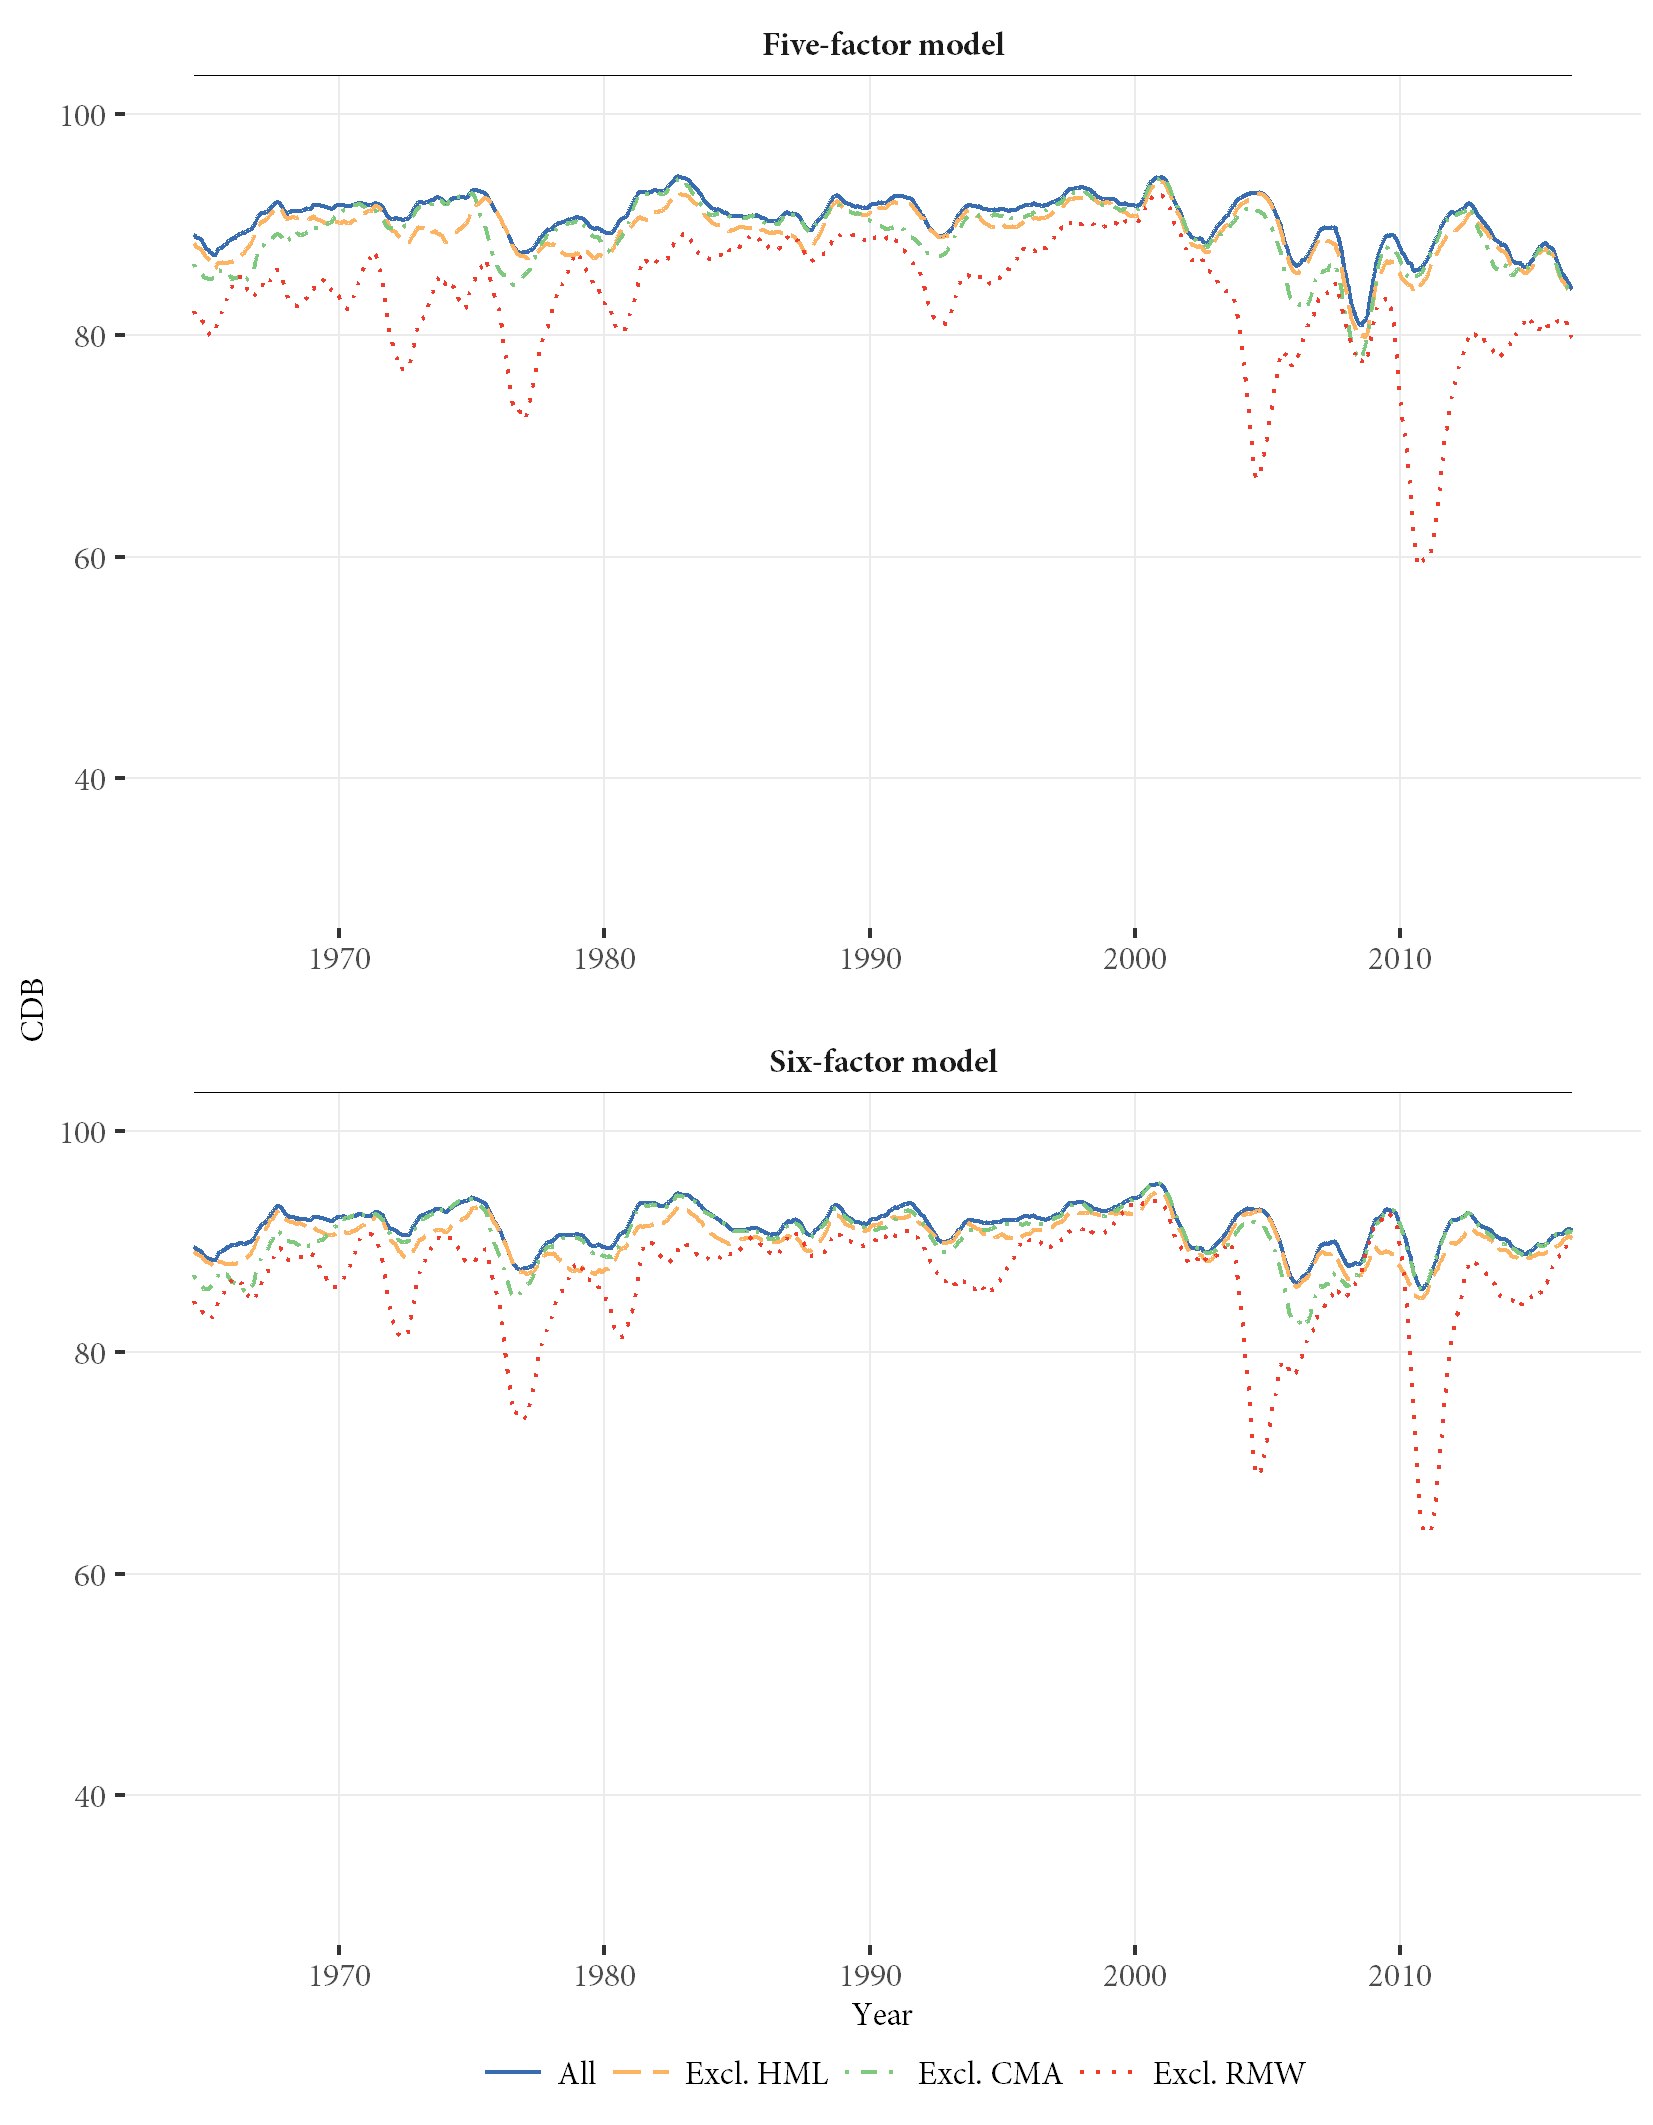
\includegraphics[scale = 1]{graphics/cdb/CDB.png}
\end{figure}

% CDB is very high; factor strategies are good diversifiers
First, we note that regardless of whether momentum is included or not, factor strategies appear to offer high levels of diversification. In absolute terms, all strategies fluctuate in the 80--95 range for the majority of the studied time period. 

% Dips
Second, there are notable dips in the diversification benefit measure. The dips represent times when diversification is relatively hard to come by, and roughly coincide in the five- and six-factor models. Interestingly, the periods of low diversification do not seem be stock market crises, as the CDB measure remains relatively high during the 1999-2000 bubble and the 2007-2009 recession.

% HML is a better diversifier on average
% CMA better when diversification is hard to come by
Third, the level decreases in diversification benefit of removing HML or CMA seem quite small. Furthermore, this decrease is highly similar; At certain times, portfolios including HML are more diversified and vice versa, but no pattern emerges. However, we note that the exclusion of RMW is dramatically different. Without RMW, the level decrease is substantial and dips in CDB become much more pronounced and frequent.

%!TEX root = ../../main.tex

\begin{table}
  \centering
  \footnotesize
  \renewcommand{\arraystretch}{1.2}

  \caption{CDB optimization with dynamic copula model (1963--2016)}

  \begin{longcaption}
    Average weights are averages of dynamic CDB optimal weights based on simulations of the return distribution from the dynamic symmetric \emph{t} copula model. Differences in average weights are expressed relative to the full five- and six-factor models. Performance measures are based on realized returns. SR is the annualized Sharpe Ratio. VaR, ES and CDB are all based on the one-week-ahead 5\% lower tail of the return distribution. Differences in CDB are to be read as column model minus row model and its associated standard errors (in parentheses) are computed taking the copula model as given.
  \end{longcaption}

  \label{tab:cdb_model}

  \begin{tabularx}{\textwidth}{@{} l dddd X dddd @{}}
    \toprule
    &
      \multicolumn{4}{c}{Five (four) factor models} &&
      \multicolumn{4}{c}{Six (five) factor models} \\
    \cmidrule{2-5}
    \cmidrule{7-10}
    &
      \multirow{2}{*}{All} &
      \multicolumn{1}{c}{Excl.} &
      \multicolumn{1}{c}{Excl.} &
      \multicolumn{1}{c}{Excl.} & &
      \multirow{2}{*}{All} &
      \multicolumn{1}{c}{Excl.} &
      \multicolumn{1}{c}{Excl.} &
      \multicolumn{1}{c}{Excl.} \\
    &
      &
      \multicolumn{1}{c}{HML} &
      \multicolumn{1}{c}{CMA} &
      \multicolumn{1}{c}{RMW} &&
      &
      \multicolumn{1}{c}{HML} &
      \multicolumn{1}{c}{CMA} &
      \multicolumn{1}{c}{RMW} \\
    \midrule
    \multicolumn{1}{@{}l}{\textbf{Average weights}} \\
    Mkt.RF & 11.1 & 10.5 & 11.5 & 19.2 & & 10.5 & 10.1  & 10.6 & 15.5 \\
    SMB    & 16.6 & 18.3 & 19.1 & 22.6 & & 15.8 & 17.9 & 18.1 & 19.2 \\
    HML    & 17.4 &      & 30.1 & 26.7 & & 18.1 &      & 28.7 & 24.9 \\
    CMA    & 21.2 & 35.0 &      & 31.6 & & 18.7 & 32.2 &      & 24.1 \\
    RMW    & 33.8 & 36.2 & 39.3 &      & & 28.1 & 31.8 & 32.6 & \\
    Mom    &      &      &      &      & &  8.8 & 8.1  & 10.0 & 16.2 \\
    \midrule
    \multicolumn{1}{@{}l}{\textbf{Difference weights}} \\
    Mkt.RF & & -0.6  & 0.4   & 8.1   & & & -0.4  & 0.2   & 5.1 \\
    SMB    & & 1.7   & 2.5   & 6.0   & & & 2.1   & 2.3   & 3.4 \\
    HML    & & -17.4 & 12.7  & 9.3   & & & -18.1 & 10.6  & 6.8 \\
    CMA    & & 13.9  & -21.2 & 10.4  & & & 13.5  & -18.7 & 5.4 \\
    RMW    & & 2.4   & 5.5   & -33.8 & & & 3.7   & 4.4   & -28.1     \\
    Mom    & &       &       &       & & & -0.7  & 1.3   & 7.5 \\
    \midrule
    \multicolumn{1}{@{}l}{\textbf{Performance}} \\
    Mean (\%)      & 2.77  & 2.94  & 2.85  & 3.37  & & 3.37  & 3.39  & 3.41  & 3.90 \\
    SD (\%)        & 2.42  & 2.49  & 2.69  & 3.89  & & 2.37  & 2.52  & 2.56  & 3.49 \\
    SR             & 1.14  & 1.18  & 1.06  & 0.87  & & 1.42  & 1.34  & 1.33  & 1.12 \\
    Avg. VaR  (\%) & 0.46  & 0.48  & 0.52  & 0.78  & & 0.45  & 0.47  & 0.49  & 0.69 \\
    Avg. ES  (\%)  & 0.61  & 0.64  & 0.69  & 1.04  & & 0.60  & 0.64  & 0.66  & 0.92 \\
    Avg. CDB       & 90.42 & 89.29 & 89.19 & 83.42 & & 91.33 & 90.24 & 90.51 & 86.62 \\
    \midrule
    \multicolumn{1}{@{}l}{\textbf{Difference CDB (column model minus row model)}} \\
    All       & & -1.13  & -1.23  & -7.01  & & & -1.09  & -0.82  & -4.71 \\
              & & (0.02) & (0.03) & (0.11) & & & (0.02) & (0.03) & (0.10) \\
    Excl. HML & &        & -0.10  & -5.88  & & &        & 0.27   & -3.62 \\
              & &        & (0.04) & (0.11) & & &        & (0.04) & (0.10) \\
    Excl. CMA & &        &        & -5.78  & & &        &        & -3.89 \\
              & &        &        & (0.11) & & &        &        & (0.10) \\
    \bottomrule
  \end{tabularx}
\end{table}


\autoref{tab:cdb_table} displays CDB summary statistics and results of paired t-tests of CDB difference between strategies (column less row strategy). This table tells largely the same story as the previous graph. In a five-factor model, excluding CMA leads to significantly lower CDB compared to excluding HML (i.e. CMA is more important as a diversifier), however, the effect is reversed in six-factor model. Furthermore, the average differences, $-0.10$ and $0.27$ respectively, are not very large -- especially compared to the effect of excluding RMW.\footnote{Standard errors are computed ignoring uncertainty in the copula model parameters, which means that the significance is overestimated.}

% \autoref{tab:cdb_table} displays CDB summary statistics and the results of paired t-tests of the differences between strategies. This table tells the same story as the graph. Excluding RMW is significantly worse for diversification than excluding either HML or CMA. For HML and CMA, differences are small: In a five-factor setting [HML] is the significantly better diversifier, while in a six-factor setting [CMA] is.\footnote{p-values are computed ignoring uncertainty in the model parameters}.

In summary, we find that the high similarity of HML and CMA indicates that tail diversification benefits are not dramatically improved by including both the factors, which is coherent with fact that they are closely related and overlap. This does not mean that both factors should not be considered, however, as it could improve the conventional risk-return tradeoff in a mean-variance setting. The RMW factor, on the other hand, is shown to be very important for diversification purposes and should be considered by all factor investors concerned with tail risk.

% What periods does low CDB correspond to?
% Story related to threshold correlations and patterns seen Mkt-HML

% No obvious corresponde with the market's performance. This does not appear
% to be related to the tail dependency so mcuh...

% subsection conditional_diversification_benefit (end)


